\chapter{Tutorials}
\label{chap:tut}

%\section[Building a slope model from scratch]{Building and simulation of a slope model using CUBIT/Trelis and SPECFEM3D\_GEOTECH}
\section{Building a slope model from scratch: Serial run}
\label{sec:cubit}

\begin{figure}[ht]
\centering
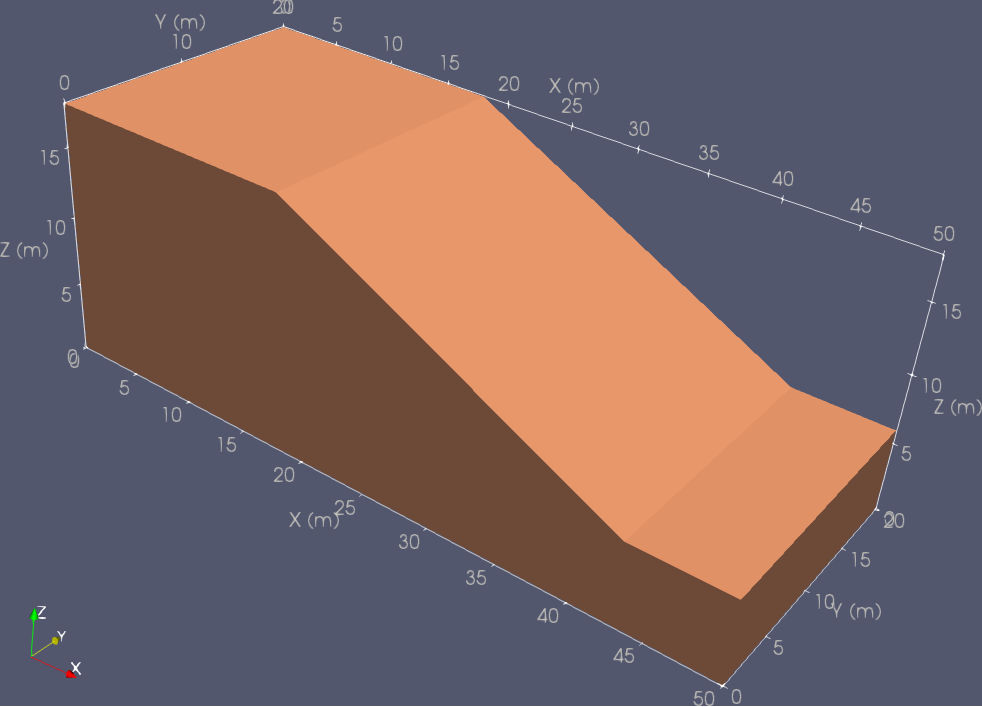
\includegraphics[scale=0.7]{cubit_example}
\caption{A slope model.}
\label{fig:slope}
\end{figure}

In this tutorial, we build a slope model as shown in Figure~\ref{fig:slope} using CUBIT/Trelis and simulate slope failure using SPECFEM3D\_GEOTECH.

\subsection*{Step 1: Create a mesh in CUBIT/Trelis}

Create a journal file "\texttt{cubit\_example.jou}" with following content:\\
\\
\colorbox{gray}{
\parbox{16cm}{
\noindent{\texttt{\#--------------BEGIN "cubit\_example.jou"----------------------------------------------\\
\# create model\\
create vertex 0 0 0\\
create vertex 50 0 0\\
create vertex 50 0 6\\
create vertex 43 0 6\\
create vertex 18 0 18\\
create vertex 0 0 18\\
create curve vertex 1 2\\
create curve vertex 2 3\\
create curve vertex 3 4\\
create curve vertex 4 5\\
create curve vertex 5 6\\
create curve vertex 6 1\\
create surface curve 1 2 3 4 5 6\\
sweep surface 1 vector 0 1 0 distance 20\\
compress all\\
\# mesh surface\\
surface 8 size 2\\
surface 8 scheme pave\\
mesh surface 8\\
\# mesh volume sweeping surface mesh\\
volume 1 size 2\\
volume 1 redistribute nodes off\\
volume 1 scheme Sweep source surface 8 target surface 1 sweep\_smooth Auto sweep\_transform least\_squares autosmooth\_target off\\
mesh volume 1\\
}}
}}
\newpage
% remaining part
\colorbox{gray}{
\parbox{16cm}{
\noindent{\texttt{\# define block\\
set duplicate block elements off\\
block 1 volume 1\\
\# define boundary conditions\\
Sideset 1 surface 2\\
sideset 1 name \sq{bottom\_ssbcux\_ssbcuy\_ssbcuz}\\
Sideset 2 surface 8\\
sideset 2 name \sq{front\_ssbcuy}\\
Sideset 3 surface 1\\
sideset 3 name \sq{back\_ssbcuy}\\
Sideset 4 surface 7\\
sideset 4 name \sq{left\_ssbcux}\\
Sideset 5 surface 3\\
sideset 5 name \sq{right\_ssbcux}\\
compress all\\
\# save and export mesh\\
save as "cubit\_example.cub" overwrite\\
set large exodus file on\\
export mesh "cubit\_example.e" overwrite\\
\#------------------END "cubit\_example.jou"---------------------------------------
}}
}}
\\
\\
Then open "\texttt{cubit\_example.jou}" file in CUBIT/Trelis and run.\\
\\
\textbf{\emph{Note}}: Above procedure can also be performed manually using CUBIT's GUI.

\subsection*{Step 2: Convert "Binary" EXODUS file to "ASCII" format}
\texttt{ncdump cubit\_example.e > cubit\_example.txt}\\

\textbf{\emph{Note}}: You must have installed NetCDF libraries. NetCDF is a free software which can be downloaded from
\texttt{http://www.unidata.ucar.edu/downloads/netcdf/index.jsp}

\subsection*{Step 3: Compile exodus2semgeotech tool}
If not already compiled, compile exodus2semgeotech.c located at \texttt{util/} folder\\
\\
\texttt{gcc exodus2semgeotech.c -o exodus2semgeotech}
\\
\\
\textbf{\emph{Note}}: For more information, please check the header in \texttt{exodus2semgeotech.c} file.

\subsection*{Step 4: Convert exodus file to SPECFEM3D\_GEOTECH files}

\texttt{./exodus2semgeotch cubit\_example.txt}\\
\\
Copy all generated files to \texttt{input/} folder.

\subsection*{Step 5: Prepare BC files}

Open BC files "\texttt{input/cubit\_example\_ssbcux}", "\texttt{input/cubit\_example\_ssbcuy}",\newline "\texttt{input/cubit\_example\_ssbcuz}". Add a line containing\\
\\
\texttt{2 0.0}\\
\\
on the top of each file and save.

\subsection*{Step 6: Create a material properties file}

Create a file "\texttt{cubit\_example\_material\_list}" in \texttt{input/} folder with the following content:
\\
\\
\colorbox{gray}{
\parbox{16cm}{
\noindent{\texttt{\# material properties (id,domain,type,gamma,ym,nu,phi,coh,psi)\\
1\\
1, 1, 0, 18.8, 1e5, 0.3, 20.0, 29.0, 0.0\\
}}
}}

\subsection*{Step 7: Create a main input file}

Create a file "\texttt{cubit\_example.sem}" in \texttt{input/} folder with the following content:
\\

\colorbox{gray}{
\parbox{16cm}{
\noindent{\texttt{\#-----------------BEGIN "cubit\_example.sem"---------------------------------------------------\\
\#pre information\\
preinfo: method=\sq{sem}, ngllx=3, nglly=3, ngllz=3, nenode=8, ngnode=8, \&\\
inp\_path=\sq{./input}, out\_path=\sq{./output/}\\
\\
\#mesh information\\
mesh: xfile=\sq{cubit\_example\_coord\_x}, yfile=\sq{cubit\_example\_coord\_y}, \&\\
zfile=\sq{cubit\_example\_coord\_z}, confile=\sq{cubit\_example\_connectivity}, \&\\
idfile=\sq{cubit\_example\_material\_id}\\
\\
\#boundary conditions\\
bc: uxfile=\sq{cubit\_example\_ssbcux}, uyfile=\sq{cubit\_example\_ssbcuy}, \&\\
uzfile=\sq{cubit\_example\_ssbcuz}\\
\\
\#material list\\
material: matfile=\sq{cubit\_example\_material\_list}\\
\\
\#control parameters\\
control: cg\_tol=1e-8, cg\_maxiter=5000, nl\_tol=0.0005, nl\_maxiter=3000, \&\\
nsrf=3, srf=1.0 1.5 2.0\\
\\
\#save data options\\
save: disp=1\\
\#-----------------END "cubit\_example.sem"---------------------------------------------------
}}
}}

\subsection*{Step 8: Run prgroam}

go to SPECFEM3D\_GEOTECH folder in terminal and type\\
\\
\texttt{./bin/semgeotech ./input/cubit\_example.sem}\\
\\
\textbf{\emph{Note}}: You must have compiled SPECFEM3D\_GEOTECH. For more detail please see Chapter~\ref{chap:start}.

\subsection*{Step 9: Visualize result}

Start ParaView. Open "\texttt{output/cubit\_example.case}" file and press "Apply" button. From "Coloring" dropdown list, select \sq{displacement} to color, and you will see the Figure~\ref{fig:disp}\\
\\
\begin{figure}[ht]
\centering
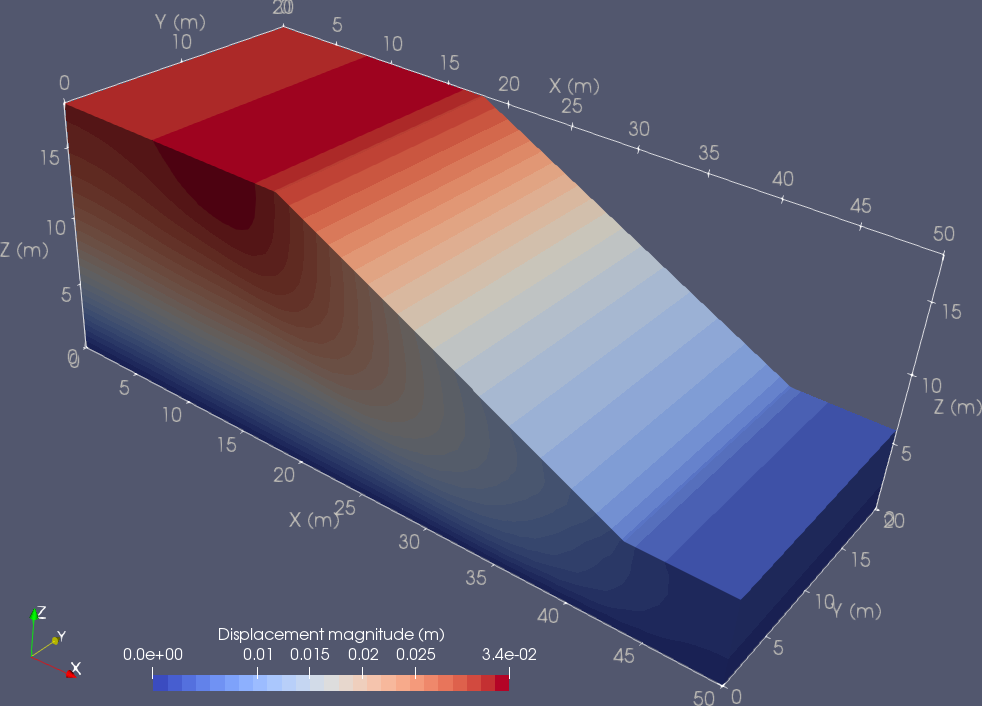
\includegraphics[scale=0.7]{cubit_example_disp}
\caption{A slope model.}
\label{fig:disp}
\end{figure}

\textbf{\emph{Note}}: You must have installed ParaView. ParaView is a free opensource visualization software which
can be downloaded from \texttt{http://www.paraview.org/}.

\section{Building a slope model from scratch: Parallel run}
\label{sec:cubit}

We can run the same model in parallel. You must have compiled the parallel version of the SPECFEM3D\_GEOTECH (See Chapter~\ref{chap:start}).\\
\\
\begin{figure}[ht]
\centering
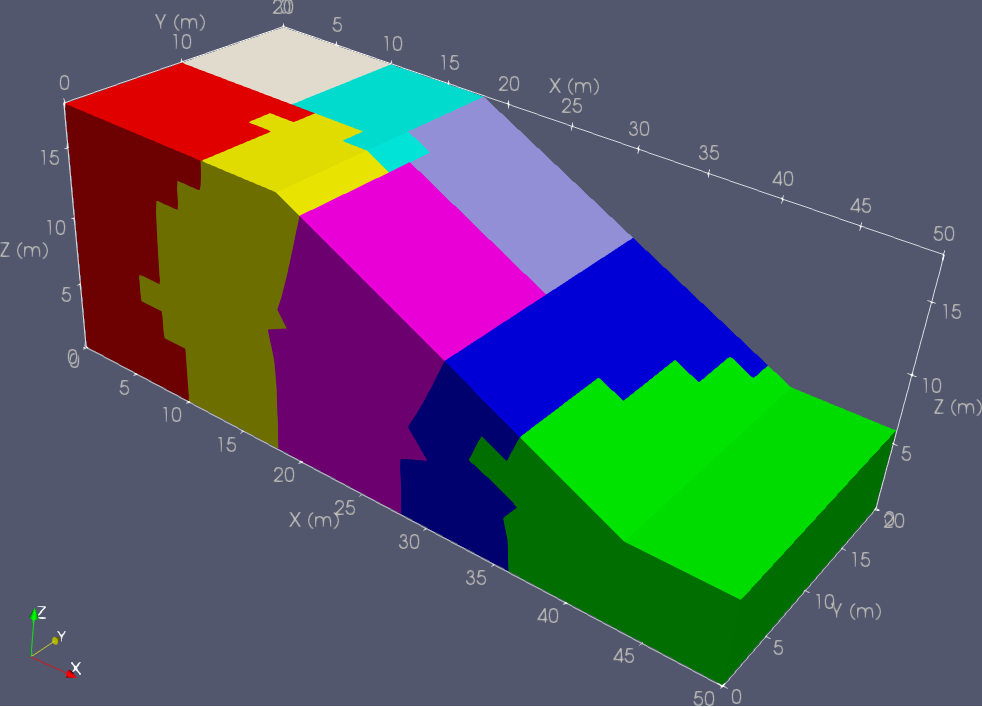
\includegraphics[scale=0.7]{cubit_example_parallel}
\caption{Eight partitioned domains of the slope model for a parallel processing.}
\label{fig:par}
\end{figure}

In this tutorial we build a slope model as shown in Figure~\ref{fig:slope} using CUBIT/Trelis and simulate slope failure using parallel SPECFEM3D\_GEOTECH.

\subsection*{Step 1 to 6: Identical to Serial run. We can follow the same Steps 1 to 6 or just use the same files produced in the serial run until the Step 6 in the serial run.}


\subsection*{Step 7: Create a main input file}

Main input files for serial and parallel runs are very similar. For the parallel run, only two additional parameters "\texttt{nproc}" in the "\texttt{preinfo:}" line and "\texttt{gfile}" in the "\texttt{mesh:}" line are needed. See Chapter~\ref{chap:input} for more details.\\
\\

Create a file "\texttt{cubit\_example.psem}" in \texttt{input/} folder with the following content:
\\

\colorbox{gray}{
\parbox{16cm}{
\noindent{\texttt{\# -----------------BEGIN "cubit\_example.psem"---------------------------------------------------\\
\#pre information\\
preinfo: nproc=8, method=\sq{sem}, ngllx=3, nglly=3, ngllz=3, nenode=8, \&\\
ngnode=8, inp\_path=\sq{./input}, out\_path=\sq{./output/}\\
\\
\#mesh information\\
mesh: xfile=\sq{cubit\_example\_coord\_x}, yfile=\sq{cubit\_example\_coord\_y}, \&\\
zfile=\sq{cubit\_example\_coord\_z}, confile=\sq{cubit\_example\_connectivity}, \&\\
idfile=\sq{cubit\_example\_material\_id}, gfile=\sq{cubit\_example\_ghost}\\
\\
\#boundary conditions\\
bc: uxfile=\sq{cubit\_example\_ssbcux}, uyfile=\sq{cubit\_example\_ssbcuy}, \&\\
uzfile=\sq{cubit\_example\_ssbcuz}\\
\\
\#material list\\
material: matfile=\sq{cubit\_example\_material\_list}\\
\\
\#control parameters\\
control: cg\_tol=1e-8, cg\_maxiter=5000, nl\_tol=0.0005, nl\_maxiter=3000, \&\\
nsrf=3, srf=1.0 1.5 2.0\\
\\
\#save data options\\
save: disp=1\\
\#-----------------END "cubit\_example.psem"---------------------------------------------------
}}
}}
\\
\\
In the above file, we have used \texttt{nproc=8}, that means we want to run the program with eight processors.

\subsection*{Step 8: Partition the mesh}

go to SPECFEM3D\_GEOTECH folder in terminal and type\\
\\
\texttt{./bin/partmesh ./input/cubit\_example.psem}\\
\\
It will produce several files in \texttt{partition/} folder.\\
\\
\textbf{\emph{Note}}: You must have compiled \texttt{partmesh} tool. For more detail please see Chapter~\ref{chap:start}.

\subsection*{Step 9: Run prgroam}

go to SPECFEM3D\_GEOTECH folder in terminal and type\\
\\
\texttt{mpirun -n 8 ./bin/psemgeotech ./input/cubit\_example.psem}\\
\\
If your cluster has the job submition system, you must use the appropriate job submission script.\\
\\

\textbf{\emph{Note}}: You must have compiled parallel SPECFEM3D\_GEOTECH. For more detail please see Chapter~\ref{chap:start}.

\subsection*{Step 10: Visualize result}

Start ParaView. Open all (Eight for this tutorial) case files "\texttt{output/cubit\_example\_proc0.case}", "\texttt{output/cubit\_example\_proc1.case}", ad so on. Press "Apply" button. From "Filters" menu select \sq{Alphabetical} $\Rightarrow$ \sq{Group Datasets}. From "Coloring" dropdown list, select \sq{displacement} to color, and you will see the Figure~\ref{fig:pardisp}\\
\\
\begin{figure}[ht]
\centering
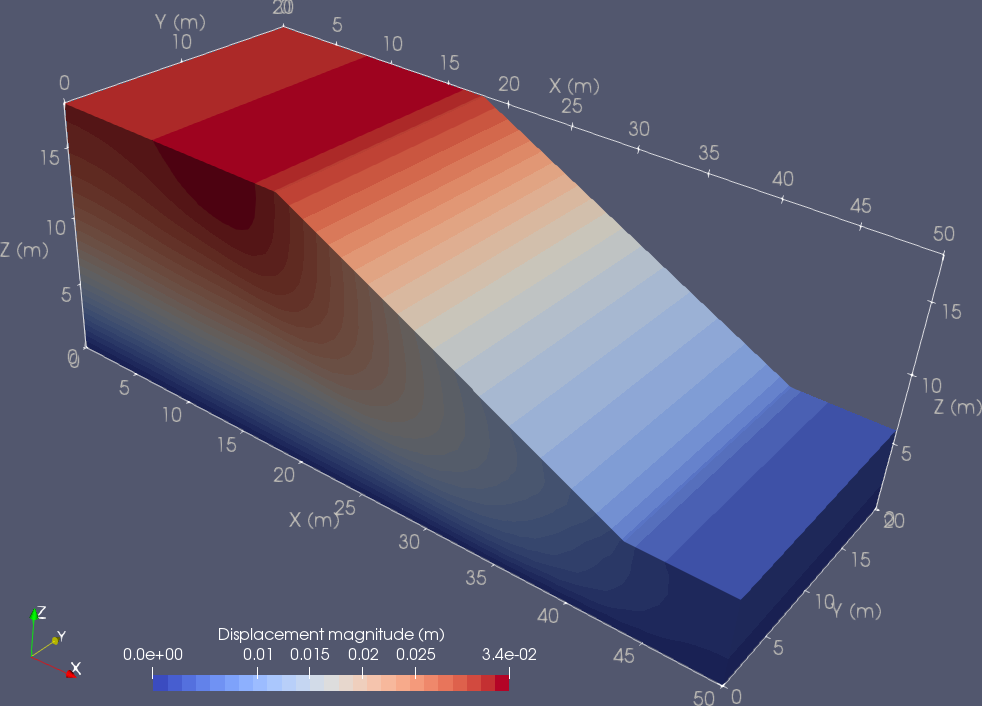
\includegraphics[scale=0.7]{cubit_example_disp}
\caption{A slope model.}
\label{fig:pardisp}
\end{figure}
\\
If the appropriate parallel version of ParaView is installed, you can visualize above results in parallel.\\
\\
\textbf{\emph{Note}}: You must have installed ParaView. ParaView is a free opensource visualization software which
can be downloaded from \texttt{http://www.paraview.org/}.\\
\\
Do you observe speedup with the parallel run? Do you get the identical results for serial and parallel run?
